\chapter{TC4合金固溶时效处理}
三种不同固溶温度得到的试样组织如下:
\begin{figure}[h!]
	\centering
	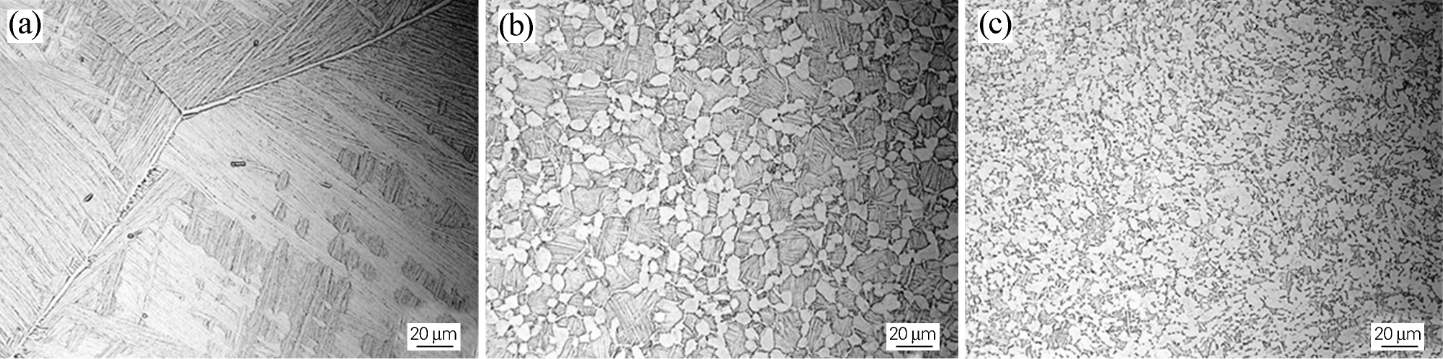
\includegraphics[width=0.7\linewidth]{pic/demo-mico}
	\caption{不同热处理工艺下 TC4 钛合金的显微组织}
	\label{fig:demo-mico}
\end{figure}

从图中经过分析可以看出:固溶-时效处理后试样对材料各方面的影响还是比较明显的。力学性能对比分析如下
\begin{enumerate}
	\item \textbf{整体塑性降低:}与对照组相比,910℃固溶组塑性大幅度降低,在经过短暂的屈服阶段后即被拉断;950℃、990℃固溶组的塑性更低,几乎呈现出来脆性材料的特点,断裂都属于脆性断裂。
	\item \textbf{抗拉强度有所提升:}910℃、950℃固溶组的抗拉强度与对照组相比都有所提升,其中以910℃固溶+510℃空冷组的强度为最高。
	\item \textbf{固溶温度较高时,强度有所降低}990℃固溶组的强度、塑性降低最为明显,990℃固溶+550℃空冷组的抗拉强度已经降低到了$ 790Mpa $左右,990℃固溶+510℃空冷组的最大应变达到了$ 2.18\% $,几乎是对照组$ 6.83\% $的三分之一。
\end{enumerate}


本设计设置的固溶处理的温度较高,在相变点附近,在高温状态下进行保温目的是为了让合金内部化学元素发生充分扩散,使成分均匀化,并发生 $\alpha\to\beta$ 转变以获得高温$ \beta $相组织。保温一段时间后,在较快冷却条件下抑制钛合金自发的$\beta\to \alpha$ 转变, 从而获得 $ \alpha^{\prime} $相马氏体、$ \alpha^{\prime\prime} $相马氏体以及亚稳$ \beta^{\prime} $相等组织。
%TC4 钛合金在稳定状态下含有少量的 β 相,β 相的存在使其具有热处理强化的能 力。由\ref{fig:tc4change}可知,固溶处理过程中固溶温度对固溶后的亚稳定相种类起决定作 用,不同固溶温度下 α 与 β 相的平衡体积分数不同,造成 β 相中合金元素含量不同, 从而在快速冷却过程中产生不同的亚稳定相。

\begin{figure}[h!]
	\centering
	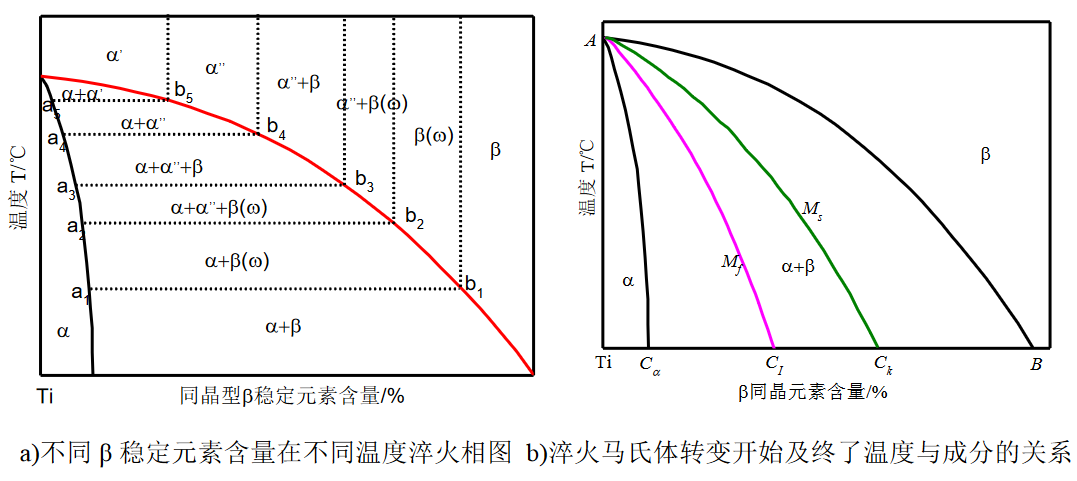
\includegraphics[width=0.7\linewidth]{pic/tc4change}
	\caption{钛合金在淬火过程中的亚稳定相及马氏体转变温度}
	\label{fig:tc4change}
\end{figure}

{\color{red}\bfseries 此处当有图形来说明转变过程}

固溶处理得到的组织可以为后续的时效处理提供良好的组织状态。本实验时效处理的温度较低,在500℃附近,通过将固溶处理后得到的亚稳态组织加热到一定温度后保温60分钟,目的是促使得到的亚稳定相在热力学作用下来降低体系的能量,使组织向稳定状态转变,产生弥散分布的析出相,来对合金起到强化作用。

在对拉伸试验的结果进行初步分析后,发现固溶与时效的处理对于合金性能的影响强度是不同的,其中以固溶处理对合金性能的影响较大,因此本实验以固溶温度为主要影响因素进行分析,将热处理的后的九组试样根据固溶温度(\textbf{510-550-590})分为三个大组来进行分析

{\color{red}\bfseries 此处当有图来证明固溶对性能影响的相强关性}

\section{相变点以下固溶处理对组织性能的影响}
本设计所用的TC4合金材料的相变点温度为973℃,前三组试样进行固溶时效的参数与性能结果如下:
{\color{purple}\bfseries 此处当有表格+图形来表示组内试样的性能参数(突出对比以便说明)}

\subsection{组织分析}
该组试样的固溶温度为910℃,在相变点以下。在处理过程中,随着温度的升高,$ \alpha $相逐渐向$ \beta $相转变,在达到设定的温度时,组织由初生等轴$ \alpha $相和$ \beta $相组成。经过水或淬火油的快速冷却后,组织发生马氏体转变,从\textbf{\large 图}可得,冷却后的组织有等轴初生$ \alpha $相和针状马氏体组成。

由于油冷情况下的冷却速度比水冷的小,组织中的初生a相的生长时间更久,形成的等轴a相尺寸较大,b相中合金元素可以发生扩散,发生扩散型相变,最终形成与珠光体类似的a片层与b片层相间分布的b转变组织,亦即双态组织;而水冷的速度比较快,本设计所用小试样的比表面积相对较大,导致冷却极快,导致b-a的扩散型相变来不及发生,b相只能通过类似马氏体相变的非扩散型晶格切变来进行相变,生成了a‘马氏体,水冷后最终组织中含有a相与a’相。

\subsection{性能分析}
该组试样的一个典型特点是固溶后的初生等轴a相含量较多,而钛合金经过固溶时效后的塑性性能指标主要取决于初生等轴a相的含量及分布\cite{zouhaibeiTC4taihejinrechuliqianghuagongyijixiangbianhangweiyanjiu2019},当初生等轴a相的含量为$ 15\%\~20\% $之间时,随着等轴a相的增加,材料的塑性逐渐增加,从图可以看出,该组材料的延伸率基本上达到了$ 3\% $以上,塑性较好。而且该组合金在

{\color{purple}\bfseries 此处添加固溶温度与a相含量关系图)}



\section{两相区固溶处理对组织性能的影响}


\section{相变点以上固溶处理对组织性能的影响}